%File: main_iclr.tex -- Nash Bargaining Preference Optimization (NBPO), ICLR 2027 version
% Ported from main_aaai.tex (AAAI 2027 submission). Content (theorems, proofs,
% tables, numbers) is unchanged; prose was revised toward a plainer register.
\documentclass{article}
\usepackage{iclr2027_conference,times}
% math_commands.tex is NOT loaded: it redefines \E, \R, \KL and conflicts
% with the macros below.
\usepackage{hyperref}
\usepackage{url}
\usepackage{graphicx}
\usepackage{amsmath}
\usepackage{amssymb}
\usepackage{amsthm}
\usepackage{booktabs}
\usepackage{algorithm}
\usepackage{algorithmic}
\usepackage{xcolor}

% ============================================================================
% Pending experiment items carried over from the AAAI cycle. The original
% timeline (supplementary Jul 31, rebuttal Oct 19-25) referred to AAAI 2027
% and must be re-planned for the ICLR 2027 schedule.
%   P0   LLM-scale covariance test (Theorem 3 at scale): noise one HH judge,
%        retrain all rules, report clean-surplus drift.
%   P0'  Nondegeneracy / conflict-regime diagnostic on the second panel.
%   P1   3 seeds + CIs, cross-judge evaluation, external benchmarks,
%        mean-length table.
%   P2   Published baselines: MaxMin-RLHF, MODPO, Rewarded Soups, RMOD.
%   P3   KS ideal-point split estimation; epsilon ablation; weight plots.
% VERIFY against training logs: stage-count numbers in the appendix
% (NBS 0.749->0.833, worst 0.710 at two stages; KS 0.867/0.773 at four stages
% vs iterated averaging 0.859/0.755).
% VERIFY: HT-MNPO naming; if HT- is our own variant of MNPO (wu2026mnpo),
% define the acronym at first use.
% NOTE: figures/safe_radar.pdf regenerated from tab:lm2 (make_safe_radar.py).
% ============================================================================

\newtheorem{theorem}{Theorem}
\newtheorem{lemma}{Lemma}
\newtheorem{proposition}{Proposition}
\newtheorem{corollary}{Corollary}
\newtheorem{assumption}{Assumption}
\newtheorem{definition}{Definition}

\newcommand{\Y}{\mathcal{Y}}
\newcommand{\F}{\mathcal{F}}
\newcommand{\G}{\mathcal{G}}
\newcommand{\U}{\mathcal{U}}
\newcommand{\KL}{\mathrm{KL}}
\newcommand{\E}{\mathbb{E}}
\newcommand{\R}{\mathbb{R}}

\title{Nash Bargaining Preference Optimization}

% Authors must not appear in the submitted version; keep \iclrfinalcopy
% commented out for submission.
\author{Anonymous authors}

%\iclrfinalcopy % Uncomment for camera-ready version, but NOT for submission.

\begin{document}
\maketitle

\begin{abstract}
Aligning a language model with conflicting preference judges requires selecting a single trade-off among them, because only one policy is deployed. Existing methods make this selection implicitly: averaging methods optimize a fixed mixture of the judges, and maxmin methods optimize the worst-case judge. We study the selection problem directly through cooperative bargaining theory. We define the utility of judge as the probability that it prefers the trained policy to the reference policy. Under this definition the disagreement point of the bargaining problem is known exactly. The classical axiomatic solutions of Nash and of Kalai and Smorodinsky then become training objectives; we call the resulting method Nash Bargaining Preference Optimization (NBPO). We prove that both solutions give every judge a strictly higher utility than the reference, are Pareto optimal, and are invariant to per-judge label noise, a covariance property that fails for both averaging and maxmin. Algorithmically, the Nash objective admits a bilinear saddle-point formulation whose dual variables converge to the bargaining weights, and the method trains from binary comparisons alone.
\end{abstract}

\section{Introduction}
\label{sec:intro}
Practical alignment involves several preference signals at once. Helpfulness, harmlessness, factuality, and domain-specific critics evaluate the same model, and they disagree \citep{bai2022training,dai2024safe}. Since a single model is deployed, alignment must commit to one point on the trade-off surface spanned by these judges. Existing methods make this commitment implicitly. Averaging methods collapse the judges into a fixed mixture and optimize its win rate \citep{wu2025sppo,zhang2025iterative}; maxmin methods optimize the worst objective \citep{chakraborty2024maxmin,son2026rmod}; per-player formulations assign each judge its own player, in part to stay within the two-player setting where last-iterate convergence is understood \citep{wu2026mnpo}. The question of which point on the trade-off surface a deployed policy should target has not been addressed directly.

We study this selection problem as the primary object. Cooperative bargaining theory is a natural framework for it: given a feasible set of jointly achievable outcomes and a status quo, which single outcome should several parties agree on? Bargaining theory answers this question axiomatically, and its two classical solutions, due to \citet{nash1950} and to \citet{kalai1975}, are characterized by properties that are directly relevant to alignment: invariance to how each judge's utility is scaled, a guarantee that no judge is left below the status quo, and stability under changes to the option set. We show that these solutions can be computed as alignment objectives, prove the guarantees they inherit, and give a practical iterative preference optimization algorithm.

The formulation rests on one modeling choice that removes the usual estimation burden. If alignment fails, the reference model is deployed unchanged, so we measure each judge's utility against the reference and take the utility of deploying the reference as the status quo. Concretely, we define the utility of a policy $\pi$ under judge $k$ as $u_k(\pi)=P_k(\pi\succ\mu)$, the probability that judge $k$ prefers $\pi$ to the reference $\mu$. By skew-symmetry of preferences, $u_k(\mu)=\tfrac12$ for every judge, so the disagreement point is $\tfrac12\mathbf 1$ and requires no estimation. The same definition makes each utility linear in the policy, which is what allows the method to train from binary comparisons alone.

Our contributions are as follows: (i) the anchored bargaining formulation of multi-judge alignment, with an exactly known disagreement point, and Nash Bargaining Preference Optimization (NBPO), the training objective it induces; (ii) a set of guarantees, namely individual rationality, Pareto optimality, and a covariance property that separates bargaining from both averaging and maxmin; (iii) a primal--dual algorithm whose dual variables are the bargaining weights and whose policy update is a single squared-loss regression on binary labels, estimating nothing beyond $K$ win rates, with a linear last-iterate convergence guarantee; and (iv) a controlled-game validation of the individual-rationality and covariance guarantees, together with two language-model panels on which the bargaining rules separate from averaging on worst-judge utility without fixing a target objective in advance.

\section{Background}
\label{sec:background}
\paragraph{Preference-based alignment.}
We work in the preference-based contextual bandit that underlies RLHF \citep{yue2012karmed,dudik2015contextual}. A prompt $x$ is drawn from $\rho$; a policy maps $x$ to a distribution $\pi(\cdot\mid x)$ over a finite response set $\Y$; and feedback is relative. A preference oracle $P:\Y\times\Y\times\mathcal{X}\to[0,1]$ returns the probability that one response is preferred to another, and is skew-symmetric,
\begin{equation}
P(y\succ y'\mid x)+P(y'\succ y\mid x)=1,\qquad P(y\succ y\mid x)=\tfrac12 .
\label{eq:skew}
\end{equation}
The oracle need not come from a scalar utility, so cyclic preferences are allowed \citep{may1954intransitivity}. For policies, $P(\pi\succ\pi'\mid x)=\E_{y\sim\pi,y'\sim\pi'}[P(y\succ y'\mid x)]$. We fix a context and drop $x$; every statement lifts by conditioning and averaging. Nash learning from human feedback \citep{munos2024nash,azar2024general} seeks a von Neumann winner through the KL-regularized game $\max_\pi\min_{\pi'}P(\pi\succ\pi')-\tau\KL(\pi\|\mu)+\tau\KL(\pi'\|\mu)$, and INPO \citep{zhang2025iterative} turns each mirror step into a regression on pairwise log-ratios that needs only binary outcomes. We are interested in alignment with $K$ oracles $P_1,\dots,P_K$; the question is what to do when they conflict.

\paragraph{Bargaining problems.}
A $K$-player bargaining problem is a pair $(\F,d)$ where $\F\subset\R^K$ is compact and convex, $d\in\F$, the set is comprehensive relative to $d$, and some $u\in\F$ has $u>d$ componentwise. A solution $f$ assigns to every such problem a point $f(\F,d)\in\F$. Coordinate $k$ of $u\in\F$ is the utility judge $k$ receives; $d$ is the disagreement point.
\citet{nash1950} proposed four axioms: Pareto optimality (PO), symmetry (SYM), scale covariance (SC, invariance to positive affine rescaling of any coordinate), and independence of irrelevant alternatives (IIA). Exactly one solution satisfies all four:
\begin{equation}
f^{\mathrm N}(\F,d)=\arg\max_{u\in\F,\,u>d}\;\sum_{k=1}^{K}\log(u_k-d_k).
\label{eq:nash}
\end{equation}
In the first-order condition of the log form, judge $k$'s direction is weighted by $1/(u_k-d_k)$, the inverse of its realized surplus, so the judge with the smallest surplus receives the largest weight while no judge's gain is driven exactly to zero. \citet{kalai1975} replace IIA by individual monotonicity (IM), which requires that expanding the feasible set while preserving all other judges' ideal utilities cannot decrease judge $k$'s utility at the selected outcome. With the ideal point $u^\ast_k=\max\{u_k:u\in\F,u\ge d\}$, their solution is the maximal feasible point on the segment from $d$ to $u^\ast$, equivalently
\begin{equation}
f^{\mathrm{KS}}(\F,d)\in\arg\max_{u\in\F}\;\min_k\frac{u_k-d_k}{u^\ast_k-d_k},
\label{eq:ks}
\end{equation}
a maximin over canonically normalized surpluses.

\section{Alignment as a Bargain Among Judges}
\label{sec:bargain}
The players are the $K$ judges. The main design question is what a judge's utility should be, and we resolve it through the disagreement point. If alignment fails, the reference $\mu$ is deployed, so a judge's utility is measured against $\mu$.

\begin{definition}[Anchored utility and surplus]
For a policy $\pi$ and judge $k$,
\begin{equation}
u_k(\pi)=P_k(\pi\succ\mu)=\textstyle\sum_y\pi(y)\,m_k(y),\qquad
s_k(\pi)=u_k(\pi)-\tfrac12,
\label{eq:anchor}
\end{equation}
with $m_k(y)=\E_{y'\sim\mu}P_k(y\succ y')$ the margin of $y$ over $\mu$.
\end{definition}

The surplus $s_k(\pi)$ is the average margin by which judge $k$ favors $\pi$ over $\mu$: a positive value means the judge prefers the trained model.

\begin{lemma}[Structure]
\label{lem:struct}
Each $u_k$ is linear in $\pi$ with values in $[0,1]$; the disagreement point is exact, $u_k(\mu)=\tfrac12$ for every $k$, so $d=\tfrac12\mathbf 1$ with no estimation; and the feasible set $\U=\{u(\pi):\pi\in\Delta(\Y)\}$ is a compact convex polytope containing $d$, whose comprehensive hull paired with $d$ is a bargaining problem whenever some policy beats $\mu$ under every judge at once.
\end{lemma}

We make three remarks. First, the exactness of the disagreement point matters: bargaining solutions are sensitive to $d$, and any error in an estimated $d$ propagates into the selected point; here skew-symmetry determines $d$ analytically. Second, the anchored definition makes each utility linear in $\pi$, which the algorithm of Section~\ref{sec:algo} converts into a training procedure whose only estimated quantities are $K$ win rates. Third, anchoring fixes $\mu$ as the standing opponent, so every objective below depends on $P_k$ only through the margins $m_k$; cyclic structure among the policy's own responses never enters. The generality of the oracle is used only at the interface: no reward model is fit, and $d$ is exact under skew-symmetry alone. The difficulty this paper addresses is the selection among judges, not the duel within a single preference.

Nothing above uses the fact that the anchor is the reference. Replacing $\mu$ by the current iterate $\pi_t$ gives the round-$t$ utilities $u^{(t)}_k(\pi)=P_k(\pi\succ\pi_t)$, and skew-symmetry again pins $d=\tfrac12\mathbf 1$ exactly, so Lemma~\ref{lem:struct} and the guarantees below hold verbatim with $\pi_t$ in place of $\mu$. Individual rationality then reads $u^{(t)}_k(\pi_{t+1})>\tfrac12$ for every $k$: each round improves every judge over the previous policy, so the iterates form a chain that is monotone judge by judge. Because a general preference oracle need not be transitive, such a chain does not by itself certify $u_k(\pi_T)>\tfrac12$ against the original reference, which is why we measure that quantity directly in the experiments.

\begin{assumption}[Nondegeneracy]
\label{ass:nondeg}
Some $\pi$ has $s(\pi)>0$ componentwise. If nondegeneracy fails, $\mu$ is already weakly Pareto optimal.
\end{assumption}

\paragraph{What existing methods select.}
Every method that deploys one policy selects one point of $\U$. Averaging solves the Nash game of a fixed mixture oracle $P_w=\sum_k w_kP_k$; since $P_w$ is skew-symmetric, that game has value exactly $\tfrac12$ regardless of the conflict, so an averaged win rate near $\tfrac12$ certifies nothing about any individual judge. In outcome space, averaging corresponds to the utilitarian point $\max\sum_k w_ku_k$, which, as we show below, can give a judge a strictly lower utility than the untrained reference. Maxmin selects the egalitarian point $\max\min_k s_k(\pi)$, which is individually rational but, because it lacks scale covariance, changes its selection when one judge's labels merely become noisier.

\paragraph{The bargaining objectives.}
For $\tau\ge0$ the Nash-bargained policy $\pi^{\mathrm N}_\tau$ and Kalai--Smorodinsky-bargained policy $\pi^{\mathrm{KS}}_\tau$ maximize
\begin{align}
J^{\mathrm N}_\tau(\pi)&=\sum_{k=1}^{K}\log s_k(\pi)-\tau\KL(\pi\|\mu),
\label{eq:jn}\\
J^{\mathrm{KS}}_\tau(\pi)&=\min_k\frac{s_k(\pi)}{u^\ast_k-\tfrac12}-\tau\KL(\pi\|\mu),
\label{eq:jks}
\end{align}
respectively, with $u^\ast_k$ the anchored ideal. Both objectives are concave: $s_k$ is affine, the log of a positive affine function is concave, a minimum of concave functions is concave, and $-\tau\KL$ is strongly concave, so $\pi^{\mathrm N}_\tau$ is unique.

\section{Theoretical Results}
\label{sec:guarantees}
All proofs, with explicit constants and witness instances, are in Appendix~\ref{app:proofs}.
\begin{theorem}[Individual rationality]
\label{thm:ir}
Under Assumption~\ref{ass:nondeg}: (i) for every $\tau\ge0$, $s_k(\pi^{\mathrm N}_\tau)>0$ for all $k$, so every judge strictly prefers the Nash-bargained policy to the reference; (ii) for every $\tau\ge0$, $s_k(\pi^{\mathrm{KS}}_\tau)>0$ for all $k$, with an explicit positive floor on the normalized surpluses; and (iii) the utilitarian (averaging) rule fails individual rationality: there are $K$-judge instances on which it selects a policy with $s_k<0$ for some judge.
\end{theorem}
The logarithmic barrier of the Nash product ensures strict individual rationality at every regularization strength $\tau$. Part (iii) shows that the failure of averaging to protect individual objectives is not merely an empirical observation: there is an explicit instance on which the utilitarian rule violates the individual-rationality axiom. Both positive parts concern the exact maximizer over $\Delta$; a parametric policy trained for finitely many stages inherits them up to optimization and estimation error, so surpluses near zero can survive training when nondegeneracy is marginal (see Section~\ref{sec:exp}).

\begin{theorem}[Pareto optimality]
\label{thm:po}
Under Assumption~\ref{ass:nondeg}, $\pi^{\mathrm N}_0$ is Pareto optimal in $(u_1,\dots,u_K)$, and for $\tau>0$, $\pi^{\mathrm N}_\tau$ is Pareto optimal in the extended vector $(u_1,\dots,u_K,-\KL(\cdot\|\mu))$.
\end{theorem}

\begin{theorem}[Covariance to judge noise]
\label{thm:cov}
Degrading judge $k$ by replacing a fraction $1-\lambda_k$ of its labels with coin flips gives the skew-symmetric oracle $P^\lambda_k=\lambda_kP_k+(1-\lambda_k)\tfrac12$. Under this compression: (i) anchored surpluses rescale exactly, $s^\lambda_k=\lambda_ks_k$, while $d$ and the KL term are unchanged, and the ideals rescale the same way; (ii) both bargaining solutions are invariant, $\pi^{\mathrm N}_\tau$ and $\pi^{\mathrm{KS}}_\tau$ are unchanged for every $\lambda\in(0,1]^K$ and $\tau\ge0$; (iii) the utilitarian and egalitarian rules are not invariant and change their selected policy under some $\lambda$.
\end{theorem}
Operationally, if one judge becomes noisier, a maxmin-aligned model drifts toward the degraded judge and an averaging-aligned model also moves, while a bargained model does not. To our knowledge this consequence of the scale covariance axiom has not been stated at the alignment level before.
% TODO(exp, P0): LLM-scale analogue of Table tab:cov. Inject label noise
% (lambda = 0.3) into one HH judge, retrain all four rules, report the drift
% of the clean surplus. This is the only empirical axis that separates NBPO
% from the egalitarian rule on clean panels.

\section{An Estimation-Free Algorithm}
\label{sec:algo}
The algorithm is a squared-loss regression on binary comparisons whose population minimizer coincides with the exact mirror update. By estimation-free we mean that no reward model, value function, or disagreement point is ever fit; the only estimated quantities in the method are the $K$ scalar win rates that the weights consume.

\paragraph{Structure of the update.}
For a fixed weight vector $\omega\in\Delta(K)$ the weighted anchored objective $\sum_k\omega_ku_k(\pi)-\tau\KL(\pi\|\mu)$ is linear in $\pi$, its opponent is the fixed reference $\mu$, and its mirror step has the closed form \eqref{eq:closed} below, with reward $r(y)=\sum_k\omega_km_k(y)$. The corresponding regression target is $\sum_k\omega_kz_k$ with per-judge binary labels
\begin{equation}
z_k=\mathbf 1[y\succ_k y'']-\mathbf 1[y'\succ_k y''],\qquad y''\sim\mu,
\label{eq:target}
\end{equation}
where one reference opponent is shared by all judges. The only additional difficulty introduced by the Nash rule is therefore the weights themselves: the first-order condition weights judge $k$ by $1/s_k$, a nonlinear function of an expectation. No estimator built from finitely many binary comparisons is unbiased for $1/s_k$, so the nonlinearity must be moved either into $K$ estimated scalars or into optimizer state.

\paragraph{Primal--dual form.}
The Fenchel identity for the logarithm, $\log s=\min_{\lambda>0}(\lambda s-\log\lambda-1)$, moves the weight into a dual variable and turns the Nash program into the bilinear saddle-point problem
\begin{equation}
\max_{\pi}\;\min_{\lambda>0}\;\sum_{k}\big(\lambda_ks_k(\pi)-\log\lambda_k-1\big)-\tau\KL(\pi\|\mu).
\label{eq:saddle}
\end{equation}
The coupling $\sum_k\lambda_ks_k(\pi)$ is bilinear, so the policy update at fixed $\lambda$ is exactly the weighted optimization step, and the dual optimum at fixed $\pi$ is $\lambda_k=1/s_k(\pi)$, the bargaining weight itself. The dual variable is not an adversary: its fixed point is the inverse-surplus bargaining vector, and the saddle is a bilinear coupling between two strongly regularized players. This is why plain mirror ascent reaches it at a linear last-iterate rate without optimism or an extragradient step (Proposition~\ref{prop:conv}).

\paragraph{From saddle to regression.}
Freeze the dual at its best response to the current policy, $\omega_{t,k}=1/s_k(\pi_t)$; normalizing these weights to the simplex, as the algorithm does, only rescales the step size $\eta_t$. One mirror-ascent step on \eqref{eq:saddle}, with the regularizer kept exact rather than linearized, is
\begin{equation}
\pi_{t+1}=\arg\max_{\pi}\;\eta_t\textstyle\sum_k\omega_{t,k}s_k(\pi)-\eta_t\tau\KL(\pi\|\mu)-\KL(\pi\|\pi_t).
\label{eq:md}
\end{equation}
Because $\sum_k\omega_{t,k}m_k$ is the gradient of $\sum_k\log s_k$ at $\pi_t$, the same step is Bregman proximal ascent on $J^{\mathrm N}_\tau$ itself (Lemma~\ref{lem:equiv}): the saddle and the concave program prescribe the same iterate. Solving the KL-proximal subproblem gives the following closed-form multiplicative reweighting:
\begin{equation}
\pi_{t+1}(y)\propto\Big(\pi_t(y)\,\mu(y)^{\eta_t\tau}\,e^{\eta_t\sum_k\omega_{t,k}m_k(y)}\Big)^{\!1/(1+\eta_t\tau)}.
\label{eq:closed}
\end{equation}
Log-ratios of \eqref{eq:closed} at a pair of responses eliminate the normalizer. Define
\begin{equation}
h_t(\pi;y,y')=\log\tfrac{\pi(y)}{\pi_t(y)}-\log\tfrac{\pi(y')}{\pi_t(y')}
+\eta_t\tau\Big(\log\tfrac{\pi(y)}{\mu(y)}-\log\tfrac{\pi(y')}{\mu(y')}\Big);
\label{eq:h}
\end{equation}
then the tilt \eqref{eq:closed} is the unique full-support policy $\pi$ satisfying $h_t(\pi;y,y')=\eta_t\sum_k\omega_{t,k}\{m_k(y)-m_k(y')\}$ at every pair, and that right side is the conditional mean of the observable target $\eta_t\sum_k\omega_{t,k}z_k$ of \eqref{eq:target}. Squared loss turns a conditional mean into a population minimizer, which closes the chain from \eqref{eq:jn} to the loss in Algorithm~\ref{alg:nbpo}.
\begin{proposition}[The regression is the mirror step]
\label{prop:exact}
Fix any weights $\omega_t\in(0,\infty)^K$, let $\pi_t$ and $\mu$ have full support, and let $\pi_{t+1}$ be \eqref{eq:closed} under these weights. Draw $y,y'\sim\pi_t$ and $y''\sim\mu$ independently with binary labels of mean $P_k$. Over full-support policies, the population minimizer of $\E\big(h_t(\pi;y,y')-\eta_t\sum_k\omega_{t,k}z_k\big)^2$ is unique and equals $\pi_{t+1}$.
\end{proposition}

\paragraph{Choice of geometry.}
The entropy geometry is necessary here, not a matter of convenience. The entropy prox is what makes \eqref{eq:md} solvable as the tilt \eqref{eq:closed}, a log-linear object that a parametric policy can match through the ratios in \eqref{eq:h}; a Euclidean step ends in a simplex projection with no expression in log-probabilities, which are the only access one has to an LLM policy. Sharing the geometry of $\KL(\pi\|\mu)$ lets the regularizer enter the subproblem exactly, which is where the $(1+\eta_t\tau)^{-1}$ pull toward $\mu$ in \eqref{eq:closed} comes from. Furthermore, the curvature of the Nash objective is controlled relative to entropy but not in the Euclidean norm: where every surplus stays above $\varepsilon$, the relative smoothness constant is $K/\varepsilon^2$ independently of $|\Y|$, while the Euclidean constant scales with $|\Y|$.
\begin{proposition}[Last-iterate convergence]
\label{prop:conv}
Let $\tau>0$, let $\varepsilon<\min_ks_k(\pi^{\mathrm N}_\tau)$, and run \eqref{eq:md} over $\Pi_\varepsilon=\{\pi:\min_ks_k(\pi)\ge\varepsilon\}$ from a full-support $\pi_0\in\Pi_\varepsilon$ with constant step $\eta\le\varepsilon^2/K$. Then $J^{\mathrm N}_\tau(\pi_t)$ is nondecreasing and
\begin{equation*}
\KL(\pi^{\mathrm N}_\tau\|\pi_T)\le(1+\eta\tau)^{-T}\KL(\pi^{\mathrm N}_\tau\|\pi_0).
\end{equation*}
\end{proposition}
The constraint is slack at the optimum by Theorem~\ref{thm:ir}, and the weight clip in the batch method below is its unconstrained surrogate: the bounded weights the analysis needs are the ones the algorithm computes anyway. The analysis starts inside $\Pi_\varepsilon$, whereas practice initializes at $\pi_0=\mu$ with $s(\mu)=0$; there the clipped weights are uniform, so the first stages run the utilitarian step and serve as the warm start into $\Pi_\varepsilon$ that Assumption~\ref{ass:nondeg} makes available.

\paragraph{Batch variant.}
Because the dual is separable and one-dimensional per judge, one can solve it to optimality each stage instead of stepping: the best response is $\lambda_{t,k}=1/\max\{\hat s_k,\varepsilon\}$, where $\hat s_k$ is judge $k$'s empirical win rate of the current batch against the cached reference batch, minus $\tfrac12$. These $K$ scalars are the only estimated quantities in the method, obtained by counting the same labels the regression consumes anyway. Algorithm~\ref{alg:nbpo} states the batch method; freezing the weights inside a stage makes the population minimizer of the squared loss exactly the mirror iterate (Proposition~\ref{prop:exact}).

\begin{algorithm}[t]
\caption{NBPO (anchored, Nash bargaining weights)}
\label{alg:nbpo}
\begin{algorithmic}[1]
\STATE \textbf{Input:} judges $P_{1:K}$ (an LLM prompted per objective, swap-averaged), reference $\mu$, $\tau$, $\varepsilon$, steps $T$.
\STATE Generate and cache a reference batch $B_\mu\sim\mu$.
\FOR{$t=0,\dots,T-1$}
  \STATE Sample $B_t\sim\pi_t$; obtain binary outcomes $\mathbf 1[y\succ_k y'']$ for $y\in B_t,y''\in B_\mu$, all $k$.
  \STATE $\hat s_k\leftarrow(\text{win rate of }B_t\text{ over }B_\mu\text{ under }k)-\tfrac12$;\; $\omega_{t,k}\propto1/\max\{\hat s_k,\varepsilon\}$.
  \STATE Form pairs $(y,y')$ from $B_t$ with shared opponents $y''\in B_\mu$; targets $\eta_t\sum_k\omega_{t,k}z_k$.
  \STATE $\pi_{t+1}\leftarrow\arg\min_\pi\widehat\E\,(h_t(\pi;y,y')-\eta_t\sum_k\omega_{t,k}z_k)^2$.
\ENDFOR
\STATE \textbf{return} $\pi_T$.
\end{algorithmic}
\end{algorithm}

\paragraph{Label sources.}
The method consumes only binary outcomes $y\succ_k y''$. A reward model yields the deterministic oracle $P_k\in\{0,\tfrac12,1\}$ by score comparison, which is skew-symmetric, so the theory applies verbatim. An LLM judge prompted with the objective rubric must be symmetrized: query both response orders and define $P_k$ as the swap-averaged verdict, since position bias otherwise breaks \eqref{eq:skew} and with it the exactness of $d=\tfrac12$. The reference batch is generated once, before training, and reused every stage, so round-robin tournaments are unnecessary.

\paragraph{KS variant.}
KS requires the normalized surpluses $\sigma_k=s_k/(u^\ast_k-\tfrac12)$, so it involves one additional estimated quantity: $u^\ast_k-\tfrac12$ is a maximum over the pool of per-response win rates. With $u^\ast$ estimated and frozen, the smoothed objective $-\beta\log\sum_k e^{-\sigma_k/\beta}-\tau\KL$ is concave, and its gradient weights $\omega_k\propto e^{-\sigma_k/\beta}/(u^\ast_k-\tfrac12)$ pass through the same regression. NBPO remains the main method; the KS variant is for practitioners who want individual monotonicity.
% TODO(exp, P3): the empirical max over the pool is upward biased for u*.
% Split-estimate it (selection half / estimation half) and report the KS
% sensitivity; add an epsilon-clip ablation and a weight-trajectory plot
% to the supplementary.

\section{Experiments}
\label{sec:exp}
The two claims that separate bargaining from averaging and maxmin, individual rationality and covariance, are exercised on a controlled preference game whose feasible set is known exactly; that check is reported in Appendix~\ref{app:toy}. Here we test whether the predicted separation survives on language-model panels, where the objectives conflict at the sample level. Throughout, NBPO-NBS and NBPO-KS name the two policies our method trains, toward the Nash and the Kalai--Smorodinsky point; both are instances of the same algorithm, and neither is a baseline.








\begin{table*}[t]
\centering\footnotesize
\setlength{\tabcolsep}{6pt}
\caption{Four-judge \textsc{HelpSteer2} panel \citep{wang2024helpsteer2}, after seven rounds of the iteration with the disagreement point re-anchored at the previous policy. Each objective is scored during training by a ground-truth reward model (the \texttt{ArmoRM} helpfulness, correctness, coherence and verbosity heads, with conciseness the negated verbosity head), which gives a deterministic skew-symmetric oracle with $d=\tfrac12$; the reference $\mu$ is a pre-alignment SFT checkpoint. Entries are anchored utilities $u_k=P_k(\pi\succ\mu)$ on held-out prompts, averaged over three independent evaluator families (\texttt{Qwen3-32B}, \texttt{Llama-3.3-70B}, \texttt{Phi-4}), none of which is the training oracle. Bold marks the best entry per column and underline the best rule that fixes no target objective in advance. The quality objectives reward length and so pull against conciseness: the preference-optimization rules bank their gains there and give up the other three, and the per-player corners take whichever objective they are told to target, at the cost of the rest. NBPO holds the highest worst-objective utility of any rule}
\label{tab:lm}
\begin{tabular}{lcccccc}
\toprule
rule & helpful & correct & coherent & concise & Avg & Worst \\
\midrule
\multicolumn{7}{@{}l}{\textit{NBPO: bargaining solutions (ours)}}\\
NBPO-KS & 0.630 & 0.607 & 0.614 & 0.616 & \underline{0.617} & \textbf{0.607} \\
NBPO-NBS & 0.633 & 0.610 & 0.614 & 0.599 & 0.614 & \underline{0.599} \\
\midrule
\multicolumn{7}{@{}l}{\textit{Nash learning from human feedback}}\\
HT-MNPO-helpful & 0.659 & 0.626 & 0.629 & 0.588 & 0.625 & 0.588 \\
HT-MNPO-correct & 0.640 & 0.612 & 0.621 & 0.598 & \underline{0.617} & 0.598 \\
HT-MNPO-coherent & \textbf{0.669} & \textbf{0.634} & \textbf{0.636} & 0.574 & \textbf{0.628} & 0.574 \\
HT-MNPO-concise & 0.231 & 0.307 & 0.265 & \textbf{0.859} & 0.415 & 0.231 \\
INPO & 0.598 & 0.582 & 0.590 & 0.654 & 0.606 & 0.582 \\
\midrule
\multicolumn{7}{@{}l}{\textit{Preference optimization}}\\
SimPO & 0.603 & 0.595 & 0.591 & 0.662 & 0.613 & 0.591 \\
IPO & 0.598 & 0.591 & 0.594 & 0.666 & 0.612 & 0.591 \\
DPO & 0.597 & 0.586 & 0.589 & 0.646 & 0.604 & 0.586 \\
\midrule
Base ($\mu$) & 0.500 & 0.500 & 0.500 & 0.500 & 0.500 & 0.500 \\
\bottomrule
\end{tabular}
\end{table*}

\paragraph{Language-model instantiation.}
On \textsc{HelpSteer2} \citep{wang2024helpsteer2} we take four objectives, helpfulness, correctness, coherence, and conciseness, and label them with a ground-truth oracle: the \texttt{ArmoRM} \citep{wang2024armorm} per-attribute heads score the two responses and the higher score wins each objective (conciseness is negated verbosity), which is deterministic, skew-symmetric, and exactly the oracle the theory assumes. Trained policies are then evaluated by a separate \texttt{Qwen3-32B} judge, so the training and evaluation oracles come from different model families and the win rates are not self-referential. Baselines span single-preference optimization (DPO \citep{rafailov2023direct}, IPO \citep{azar2024general}, SimPO \citep{meng2024simpo}), INPO on the uniform mixture oracle \citep{zhang2025iterative}, and the per-player corners of HT-MNPO \citep{wu2026mnpo}, one run per target objective; all train on the same comparisons and differ only in the per-objective weight.

Because the quality objectives reward longer answers, they conflict with conciseness, and the table shows how each family resolves that conflict. The preference-optimization rules and INPO push conciseness to $0.65$--$0.67$ and leave the other three near $0.59$; the per-player corners lift whichever objective they are given and give up the rest, most starkly the conciseness corner, which reaches $0.859$ there and falls to $0.231$ elsewhere. The bargaining rules spread the gain instead, and NBPO-KS ends with the highest worst-objective utility of any rule in the table. Its softmin temperature is read off the stage-one conflict strength rather than tuned.

\paragraph{A second panel.}
A second panel probes the opposite regime. On \textsc{SafeRLHF} \citep{dai2024safe} we score helpfulness and harmlessness with the ground-truth Beaver reward and cost models and evaluate with the same three judges. Here the two objectives largely improve together rather than conflict, and the picture changes accordingly (Table~\ref{tab:lm2}): the aggregate rules stay within a few points of the bargaining ones, SimPO taking the average at $0.818$ against $0.803$, while NBPO-KS still holds the highest worst-objective utility at $0.799$. Bargaining neither helps much nor hurts when there is little tension to arbitrate, which is the boundary the theory draws. What the panel does show sharply is the cost of naming the wrong objective in advance: the helpfulness corner reaches $0.556$ on its own target and $0.358$ on safety.


\begin{table}[t]
\centering\footnotesize
\setlength{\tabcolsep}{3pt}
\caption{Second panel on \textsc{SafeRLHF} \citep{dai2024safe}, scored during training by the ground-truth Beaver reward (helpfulness) and cost (harmlessness) models and evaluated, as in Table~\ref{tab:lm}, by averaging each objective's win rate over three independent evaluator families (\texttt{Qwen3-32B}, \texttt{Llama-3.3-70B}, \texttt{Phi-4}). Entries are $u_k=P_k(\pi\succ\mu)$ against an SFT reference; Avg is their mean, Worst their minimum, bold marks the best per column and underline the second best. The two objectives here largely improve together, so there is little for bargaining to arbitrate and the aggregate rules stay close: SimPO takes the average, while NBPO-KS still holds the highest worst-objective utility. The helpfulness corner shows what naming the wrong objective costs on a safety panel.}
\label{tab:lm2}
\begin{tabular}{lcccc}
\toprule
rule & helpful & harmless & Avg & Worst \\
\midrule
\multicolumn{5}{@{}l}{\textit{NBPO: bargaining solutions (ours)}}\\
NBPO-KS & \textbf{0.808} & 0.799 & 0.803 & \textbf{0.799} \\
NBPO-NBS & 0.762 & 0.707 & 0.735 & 0.707 \\
\midrule
\multicolumn{5}{@{}l}{\textit{Nash learning from human feedback}}\\
HT-MNPO-helpful & 0.556 & 0.358 & 0.457 & 0.358 \\
HT-MNPO-harmless & 0.754 & 0.837 & 0.795 & 0.754 \\
INPO & 0.742 & 0.838 & 0.790 & 0.742 \\
\midrule
\multicolumn{5}{@{}l}{\textit{Preference optimization}}\\
SimPO & \underline{0.787} & \textbf{0.849} & \textbf{0.818} & \underline{0.787} \\
IPO & 0.750 & 0.835 & 0.792 & 0.750 \\
DPO & 0.746 & \underline{0.844} & \underline{0.795} & 0.746 \\
\midrule
Base ($\mu$) & 0.500 & 0.500 & 0.500 & 0.500 \\
\bottomrule
\end{tabular}
\end{table}
\begin{figure}[t]
\centering
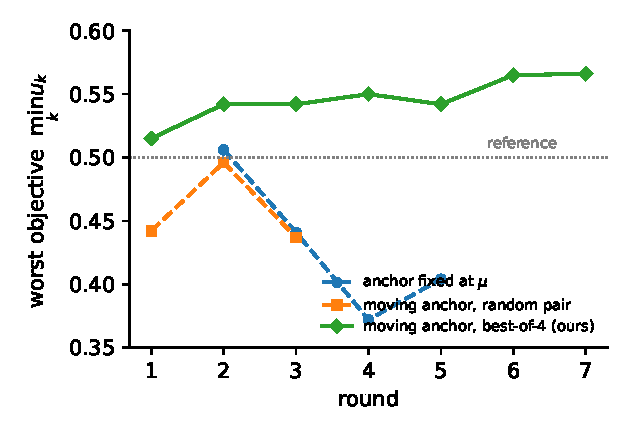
\includegraphics[width=0.62\linewidth]{figures/ablation_rounds.pdf}
\caption{What the two design choices buy, on \textsc{HelpSteer2} under \texttt{Qwen3-32B}. Anchoring every round at the reference makes the weights chase whichever objective is currently worst against $\mu$, and the iteration gives back what it just repaired. Moving the anchor to the previous policy is not enough on its own: with a random pair of the anchor's samples the round direction is too noisy and the swing persists. Selecting, among four samples, the pair with the largest weighted margin makes each round decisive, and the worst objective rises monotonically and stays above the reference.}
\label{fig:ablation}
\end{figure}

\begin{table}[t]
\centering\footnotesize
\caption{Softmin temperature of the Kalai--Smorodinsky weights, one round on \textsc{HelpSteer2}. The temperature traces the frontier between the two corners: small values concentrate weight on the objective that is worst against $\mu$ and protect it, large values approach uniform weighting and buy a little average utility by giving that objective up. We set it from the stage-one conflict strength rather than tuning it against the evaluation.}
\label{tab:beta}
\begin{tabular}{lccccc}
\toprule
$\beta$ & 0.03 & 0.05 & 0.08 & 0.12 & 0.25 \\
\midrule
Avg & 0.517 & 0.522 & 0.527 & 0.524 & 0.531 \\
Worst & \textbf{0.499} & 0.423 & 0.356 & 0.322 & 0.304 \\
\bottomrule
\end{tabular}
\end{table}

\begin{table}[t]
\centering\footnotesize
\caption{Seed replication of the four closest contenders, mean and standard deviation over training seeds at round six. These runs are scored by \texttt{Qwen3-32B} only, so they measure seed noise rather than judge robustness, and they should be read against Table~\ref{tab:lm}, whose entries average over three judges. Seed noise is small, at most $0.004$ on either column. Under this single judge the correctness corner leads on the worst objective; averaging over the three judges reverses that ordering, which is the point Section~\ref{sec:exp} makes about reading a corner result off one judge.}
\label{tab:seeds}
\begin{tabular}{lccc}
\toprule
rule & Avg & Worst & seeds \\
\midrule
NBPO-KS & $0.580\pm0.002$ & $0.561\pm0.004$ & 3 \\
NBPO-NBS & $0.581\pm0.002$ & $0.557\pm0.001$ & 2 \\
HT-MNPO-correct & $0.586\pm0.002$ & $0.575\pm0.002$ & 2 \\
SimPO & $0.575\pm0.002$ & $0.545\pm0.004$ & 3 \\
\bottomrule
\end{tabular}
\end{table}

\paragraph{Seed sensitivity.}
Table~\ref{tab:seeds} repeats the four closest contenders across training seeds. The runs are stable: the standard deviation is at most $0.004$ on either column, so the differences discussed above are not seed noise. They also isolate what a single judge decides. Scored by \texttt{Qwen3-32B} alone the correctness corner holds the best worst-objective utility, $0.575$ against $0.561$ for NBPO-KS, a gap several standard deviations wide; averaging over the three judges in Table~\ref{tab:lm} reverses it. The judge, not the seed, is what this comparison is sensitive to.

\paragraph{What the design choices buy.}
Figure~\ref{fig:ablation} isolates the two ingredients. Re-anchoring at $\mu$ every round is the natural reading of the formulation, and it fails: the minimum utility falls from $0.506$ to $0.372$ over three rounds as each round surrenders the objective the previous one repaired. Moving the anchor to the previous policy fixes the target but not the noise, and with a random pair of the anchor's samples the swing persists ($0.442$, $0.496$, $0.437$). Keeping the pair with the largest weighted margin among four samples makes the round direction consistent, and the worst objective climbs monotonically to $0.566$. Table~\ref{tab:beta} varies the softmin temperature over a single round and shows the frontier it controls, from protecting the worst-off objective at $\beta=0.03$ to approaching uniform weighting at $\beta=0.25$.

\paragraph{Balance across judges.}
The primal--dual iteration of Algorithm~\ref{alg:nbpo} is what buys this balance: re-estimating the weights each round pulls the neglected objective back up, so the bargaining policy ends balanced rather than specialized. On \textsc{HelpSteer2} a single such round is enough for NBPO-KS to clear every objective above the reference, the individual rationality and Pareto optimality of Theorems~\ref{thm:ir} and~\ref{thm:po}, realized without hand-tuning a single weight.

\section{Related Work}
\label{sec:related}
Nash learning from human feedback and its self-play instantiations optimize against a worst-case opponent for a single preference \citep{munos2024nash,wu2025sppo,zhang2025iterative}; EGPO \citep{zhou2025egpo} sharpens the last-iterate rate. Robust multi-objective methods optimize the worst objective in training or at decoding time \citep{chakraborty2024maxmin,son2026rmod}, and per-oracle formulations assign each judge a player \citep{wu2026mnpo}; all of these correspond to the egalitarian or per-player points of our feasible set. Nash welfare aggregation has been studied over learned scalar rewards \citep{zhong2024nashwelfare}, but without anchoring, an exactly known disagreement point, or an axiomatic treatment over preference oracles; social choice has also been argued to be the right lens for aggregating diverse feedback \citep{conitzer2024social}. Scalarization-based multi-objective alignment tunes or conditions on a weight vector \citep{zhou2024beyond,rame2023rewarded,wang2024arithmetic,zhong2024panacea}; there the weights are an input, whereas here they are the output of the selection. Bargaining solutions have been used in gradient-space multi-task learning \citep{navon2022nashmtl}, and \citet{han2026fair} recover Kalai--Smorodinsky from relative improvement in group-fair prediction; neither operates in outcome space over preference oracles, where anchoring makes the disagreement point exact, and Kalai--Smorodinsky has not previously appeared in the alignment literature.
% TODO(exp, P2): run the published baselines behind these citations, not only
% the in-framework corners: MaxMin-RLHF (original recipe), MODPO, Rewarded
% Soups, and RMOD at decode time.
Our contribution is to treat the selection among these points as an axiomatic problem, and to train to the selected point with an algorithm that estimates nothing beyond $K$ win rates.

\section{Conclusion}
\label{sec:conclusion}
We asked which policy the $K$ judges would jointly agree to deploy. Anchoring utilities at the reference turns multi-judge alignment into a bargaining problem with an exactly known disagreement point, on which the Nash and Kalai--Smorodinsky solutions become concave training objectives with individual rationality, Pareto optimality, and a covariance property that averaging and maxmin both lack. The Nash objective admits a bilinear saddle-point formulation whose dual variables are the bargaining weights, so the method trains from binary comparisons alone through a single regression. In a controlled preference game the bargaining solutions raise every objective above the reference where averaging sacrifices one, and remain invariant to label noise where averaging and maxmin drift. On two language-model panels whose judges genuinely conflict at the sample level, the bargaining rules keep every judge well above the reference where averaging sacrifices the worst-off one, which is the separation the theory predicts.

\subsection*{AI use statement}
% REQUIRED at ICLR 2027; does not count toward the page limit.
% FILL IN HONESTLY before submission. Describe the actual use of generative
% AI in this work (e.g., writing assistance, code assistance, literature
% search), what was not AI-assisted, and how AI-assisted content was
% verified by the authors. See the ICLR 2027 AI Policy for Authors.
In this work, we used generative AI tools for [TO BE COMPLETED BY THE AUTHORS]. We have reviewed all AI-assisted content, and we take responsibility for the final content of this work, including text, claims, and artifacts produced with the aid of generative AI.

\subsection*{Ethics statement}
This work studies methods for aligning language models with multiple preference objectives, including harmlessness. No method for causing harm is described. The datasets used (\textsc{HelpSteer2}, \textsc{SafeRLHF}) are publicly available and were used under their respective licenses.

\subsection*{Reproducibility statement}
Complete proofs of all theoretical results, with explicit constants and witness instances, are given in Appendix~\ref{app:proofs}. Appendix~\ref{app:labeling} specifies the judge instantiation, the verbatim judging prompt, the construction of training targets from verdicts, and the response-length analysis. Algorithm~\ref{alg:nbpo} states the training procedure in full, and Section~\ref{sec:exp} describes the controlled preference game in enough detail to reproduce Tables~\ref{tab:ir} and~\ref{tab:cov} exactly.

\bibliography{iclr2027_conference}
\bibliographystyle{iclr2027_conference}

\appendix
\section{Proofs}
\label{app:proofs}
Throughout, $\Y$ is finite, $\Delta=\Delta(\Y)$, and $\mu$ has full support (Assumption~\ref{ass:nondeg}), so $\KL(\pi\|\mu)\le\log(1/\min_y\mu(y))<\infty$ for every $\pi\in\Delta$. We use the convention $\log s=-\infty$ for $s\le0$ and write $\chi^2(\pi\|\mu)=\sum_y(\pi(y)-\mu(y))^2/\mu(y)$. The negative entropy is $\psi(\pi)=\sum_y\pi(y)\log\pi(y)$, so that $\KL(\pi\|\nu)=\psi(\pi)-\langle\pi,\log\nu\rangle$ for full-support $\nu$, and $\KL(x\|y)=\psi(x)-\psi(y)-\langle\nabla\psi(y),x-y\rangle$ whenever $y$ has full support.

\subsection{Proof of Lemma~\ref{lem:struct}}
\begin{proof}
Recall $m_k(y)=\E_{y'\sim\mu}P_k(y\succ y')$ and $u_k(\pi)=\sum_y\pi(y)m_k(y)$. Since $P_k$ takes values in $[0,1]$, so does each $m_k(y)$, and $u_k(\pi)$ is a convex combination of these numbers: it is linear in $\pi$ and lies in $[0,1]$.

\emph{The disagreement point.} Taking $\pi=\mu$ and unfolding the two expectations, with $y,y'$ independent draws from $\mu$,
\[
u_k(\mu)=\sum_y\mu(y)\,m_k(y)=\E_{y\sim\mu}\E_{y'\sim\mu}P_k(y\succ y')=\E_{(y,y')\sim\mu\otimes\mu}P_k(y\succ y').
\]
Because $(y',y)$ has the same law $\mu\otimes\mu$ as $(y,y')$, relabelling the two coordinates gives $\E_{\mu\otimes\mu}P_k(y\succ y')=\E_{\mu\otimes\mu}P_k(y'\succ y)$, so each of them equals half of their sum:
\[
u_k(\mu)=\tfrac12\,\E_{(y,y')\sim\mu\otimes\mu}\big[P_k(y\succ y')+P_k(y'\succ y)\big]=\tfrac12,
\]
since skew-symmetry \eqref{eq:skew} makes the bracket equal to $1$ for every pair, including $y=y'$. Hence $d=u(\mu)=\tfrac12\mathbf 1$ exactly, with nothing left to estimate.

\emph{The feasible set.} $\U=\{u(\pi):\pi\in\Delta\}$ is the image of the simplex under the linear map $\pi\mapsto u(\pi)$. A linear image of a compact convex polytope is again one, so $\U$ is a compact convex polytope, and $d=u(\mu)\in\U$.

\emph{The bargaining problem.} Let $\G=\{u'\in\R^K:d\le u'\le u\ \text{componentwise for some }u\in\U\}$; we check the four clauses. \emph{Convex}: if $d\le u'_i\le u_i\in\U$ for $i=1,2$ and $\lambda\in[0,1]$, then $\lambda u'_1+(1-\lambda)u'_2$ lies between $d$ and $\lambda u_1+(1-\lambda)u_2$, and the latter belongs to $\U$ because $\U$ is convex. \emph{Compact}: $\G\subseteq[0,1]^K$ is bounded since $\U$ is; and if $u'_n\to u'$ with $d\le u'_n\le u_n\in\U$, then compactness of $\U$ gives a subsequence $u_n\to u\in\U$, and passing to the limit in both inequalities yields $d\le u'\le u$, so $\G$ is closed. \emph{Comprehensive relative to $d$}: immediate from the definition, since lowering any coordinate of a point of $\G$ while staying above $d$ preserves membership. \emph{Nondegenerate}: $\G$ contains a point $u'>d$ if and only if some $u\in\U$ satisfies $u>d$, because $u'\in\G$ is dominated by such a $u$ and conversely any such $u$ lies in $\G$; and $u(\pi)>d$ says exactly that $s(\pi)>0$, one judge at a time, which is Assumption~\ref{ass:nondeg}. Therefore $(\G,d)$ is a bargaining problem in the sense of Section~\ref{sec:background}.
\end{proof}

\subsection{Proof of Theorem~\ref{thm:ir}}
The proof of part (ii) uses a quadratic bound on the divergence cost of mixing toward $\mu$.
\begin{lemma}\label{lem:mix}
For $\bar\pi\in\Delta$, $\pi_t=(1-t)\mu+t\bar\pi$, and $t\in[0,1]$,
$\KL(\pi_t\|\mu)\le t^2\chi^2(\bar\pi\|\mu)$.
\end{lemma}
\begin{proof}
Let $r=\bar\pi/\mu-1$, so $\pi_t=\mu(1+tr)$ and $\sum_y\mu r=0$. With $\log(1+x)\le x$,
\[
\KL(\pi_t\|\mu)=\sum_y\mu(1+tr)\log(1+tr)\le\sum_y\mu(1+tr)\,tr=t^2\sum_y\mu r^2,
\]
and $\sum_y\mu r^2=\chi^2(\bar\pi\|\mu)$.
\end{proof}

\begin{proof}[Proof of Theorem~\ref{thm:ir}]
Let $\bar\pi$ be the policy of Assumption~\ref{ass:nondeg} and fix $\tau\ge0$.

\emph{(i)} Set $c=J^{\mathrm N}_\tau(\bar\pi)>-\infty$. Every $\pi$ with $J^{\mathrm N}_\tau(\pi)\ge c$ obeys, for each $k$,
\[
\log s_k(\pi)=J^{\mathrm N}_\tau(\pi)+\tau\KL(\pi\|\mu)-\sum_{j\ne k}\log s_j(\pi)\ \ge\ c+(K-1)\log2,
\]
using $\KL\ge0$ and $s_j\le\tfrac12$, hence
\[
s_k(\pi)\ \ge\ \delta:=2^{K-1}e^{-\tau\KL(\bar\pi\|\mu)}\prod_{j}s_j(\bar\pi)\ >\ 0.
\]
So $\sup_\Delta J^{\mathrm N}_\tau$ equals the supremum over the compact set $\{\pi:s(\pi)\ge\delta\}$, on which $J^{\mathrm N}_\tau$ is continuous; a maximizer therefore exists, and every maximizer satisfies $J^{\mathrm N}_\tau\ge c$ and inherits the floor $s_k\ge\delta$ for all $k$.

\emph{(ii)} Nondegeneracy gives $s^\ast_k:=u^\ast_k-\tfrac12\ge s_k(\bar\pi)>0$, so the normalized surpluses $\sigma_k=s_k/s^\ast_k$ are continuous and $J^{\mathrm{KS}}_\tau$ attains its maximum on $\Delta$. Let $a=\min_k\sigma_k(\bar\pi)>0$ and $\chi^2=\chi^2(\bar\pi\|\mu)$, finite by full support of $\mu$ and nonzero because $s(\mu)=0\ne s(\bar\pi)$ forces $\bar\pi\ne\mu$. Each $s_k$ is affine with $s_k(\mu)=0$, so along $\pi_t=(1-t)\mu+t\bar\pi$ we have $\sigma_k(\pi_t)=t\,\sigma_k(\bar\pi)\ge ta$, and by optimality and Lemma~\ref{lem:mix},
\[
J^{\mathrm{KS}}_\tau(\pi^{\mathrm{KS}}_\tau)\ \ge\ \max_{t\in[0,1]}\big(ta-\tau t^2\chi^2\big)\ \ge\ \min\Big\{\frac a2,\;\frac{a^2}{4\tau\chi^2}\Big\},
\]
the two cases being $t=1$ when $\tau\le a/(2\chi^2)$ and $t=a/(2\tau\chi^2)$ otherwise. Since $-\tau\KL\le0$, the same number bounds $\min_k\sigma_k(\pi^{\mathrm{KS}}_\tau)$ from below. This is the claimed floor, and it is strictly positive for every $\tau\ge0$.

\emph{(iii)} Let $\Y=\{a,b\}$, write $p=\pi(a)$, and take
\[
m_1=(1,\,0.45),\qquad m_2=(0.4,\,0.55),
\]
and $m_k=(0.6,\,0.6)$ for $k\ge3$, so that $s_1=0.55p-0.05$, $s_2=0.05-0.15p$, and $s_k\equiv0.1$ for $k\ge3$. The policy $p=0.2$ has $s=(0.06,\,0.02,\,0.1,\dots)>0$, so Assumption~\ref{ass:nondeg} holds. The equal-weight utilitarian objective $\sum_ks_k(\pi)=0.4p+0.1(K-2)$ is uniquely maximized at the vertex $p=1$, where $s_2=-0.1<0$: the rule selects a policy that judge~2 strictly disprefers to the reference. For an arbitrary fixed weight vector $w>0$, the family $m_1=(1,\tfrac12-\gamma)$, $m_2=(\tfrac12-\beta,\tfrac12+\beta)$ with $\gamma,\beta>0$ and $\beta$ small relative to $w_1/w_2$ behaves identically.
\end{proof}

\subsection{Proof of Theorem~\ref{thm:po}}
\begin{proof}
By Theorem~\ref{thm:ir}(i), every maximizer under discussion has $s(\pi)>0$, so all logarithms below are finite.

\emph{Case $\tau=0$.} Suppose $u(\pi')\ge u(\pi^{\mathrm N}_0)$ coordinatewise with strict inequality at some $j$. Then $s_k(\pi')\ge s_k(\pi^{\mathrm N}_0)>0$ for all $k$ and $s_j(\pi')>s_j(\pi^{\mathrm N}_0)$, so strict monotonicity of the logarithm gives $\sum_k\log s_k(\pi')>\sum_k\log s_k(\pi^{\mathrm N}_0)$, contradicting optimality.

\emph{Case $\tau>0$.} Write $\pi^\ast=\pi^{\mathrm N}_\tau$. Suppose $u(\pi')\ge u(\pi^\ast)$ and $\KL(\pi'\|\mu)\le\KL(\pi^\ast\|\mu)$, with at least one of these $K+1$ inequalities strict. If a strict one is some $u_j$, then $\sum_k\log s_k$ increases strictly while $-\tau\KL$ does not decrease; if it is the divergence, then $-\tau\KL$ increases strictly, here $\tau>0$, while $\sum_k\log s_k$ does not decrease. Either way $J^{\mathrm N}_\tau(\pi')>J^{\mathrm N}_\tau(\pi^\ast)$, a contradiction.

\emph{Welfare loss.} Let $W=\sum_k\log s_k$. Optimality of $\pi^{\mathrm N}_\tau$ against the competitor $\pi^{\mathrm N}_0$ gives $W(\pi^{\mathrm N}_\tau)-\tau\KL(\pi^{\mathrm N}_\tau\|\mu)\ge W(\pi^{\mathrm N}_0)-\tau\KL(\pi^{\mathrm N}_0\|\mu)$, hence
\[
W(\pi^{\mathrm N}_0)-W(\pi^{\mathrm N}_\tau)\ \le\ \tau\,\KL(\pi^{\mathrm N}_0\|\mu),
\]
which is finite because $\mu$ has full support.
\end{proof}

\subsection{Proof of Theorem~\ref{thm:cov}}
\begin{proof}
\emph{(i)} From $P^\lambda_k=\lambda_kP_k+(1-\lambda_k)\tfrac12$ and the definitions, $m^\lambda_k(y)=\lambda_km_k(y)+(1-\lambda_k)\tfrac12$, hence $u^\lambda_k(\pi)=\lambda_ku_k(\pi)+(1-\lambda_k)\tfrac12$ and $s^\lambda_k=\lambda_ks_k$; in particular $u^\lambda_k(\mu)=\tfrac12$, so the disagreement point is unchanged, and the KL term never referenced the labels. For the ideals, $\{\pi:s^\lambda(\pi)\ge0\}=\{\pi:s(\pi)\ge0\}$ because every $\lambda_k>0$, so $s^{\ast,\lambda}_k=\max\{\lambda_ks_k(\pi):s(\pi)\ge0\}=\lambda_ks^\ast_k$.

\emph{(ii)} The domains coincide, $\{s^\lambda>0\}=\{s>0\}$. On them,
\[
J^{\mathrm N,\lambda}_\tau=\sum_k\log(\lambda_ks_k)-\tau\KL=J^{\mathrm N}_\tau+\sum_k\log\lambda_k,
\]
a constant shift, while $\sigma^\lambda_k=\lambda_ks_k/(\lambda_ks^\ast_k)=\sigma_k$ gives $J^{\mathrm{KS},\lambda}_\tau=J^{\mathrm{KS}}_\tau$ identically. The maximizer sets therefore coincide for every $\lambda\in(0,1]^K$ and $\tau\ge0$.

\emph{(iii)} Take $\Y=\{a,b\}$, $K=2$, $m_1=(1,\,0)$, $m_2=(0.2,\,0.9)$, and write $p=\pi(a)$, so $s_1=p-\tfrac12$ and $s_2=0.4-0.7p$. The policy $p=0.55$ has $s=(0.05,\,0.015)>0$, so Assumption~\ref{ass:nondeg} holds. The equal-weight utilitarian objective $s_1+s_2=0.3p-0.1$ selects $p=1$; degrading judge~1 with $\lambda_1=0.1$ turns it into $0.1s_1+s_2=0.35-0.6p$, which selects $p=0$. The egalitarian rule: $s_1$ increases and $s_2$ decreases in $p$, so the maximin sits at the crossing $p-\tfrac12=0.4-0.7p$, that is $p=9/17$; after the same degradation the crossing $0.1(p-\tfrac12)=0.4-0.7p$ moves to $p=9/16$. Both rules change their selected policy, while by part (ii) neither bargaining solution moves. For $K>2$, append judges with $m_k=(0.6,\,0.6)$: their constant surplus $0.1$ shifts the utilitarian objective by a constant and exceeds both maximin values, $1/34$ and $1/160$, so the added coordinates never bind. Since degrading labels by $\lambda$ rescales each surplus coordinate by $\lambda_k$, the instance also witnesses the crossed scale-covariance.
\end{proof}

\subsection{Closed form of the update and proof of Proposition~\ref{prop:exact}}
\begin{lemma}[Dual best response is the gradient weighting]\label{lem:equiv}
Fix $\pi_t$ with $s(\pi_t)>0$. The inner minimization of \eqref{eq:saddle} at $\pi_t$ is separable across $k$ with unique solution $\lambda_k=1/s_k(\pi_t)=\omega_{t,k}$, and with $f=\sum_k\log s_k$,
\[
\sum_k\omega_{t,k}m_k=\nabla f(\pi_t),
\]
so \eqref{eq:md} is the Bregman proximal step on $J^{\mathrm N}_\tau=f-\tau\KL(\cdot\|\mu)$ that linearizes $f$ at $\pi_t$ and keeps the regularizer exact.
\end{lemma}
\begin{proof}
$\partial_{\lambda_k}(\lambda_ks_k-\log\lambda_k)=s_k-1/\lambda_k$ vanishes only at $\lambda_k=1/s_k$, a minimum by convexity in $\lambda_k$. Since $s_k(\pi)=\langle\pi,m_k\rangle-\tfrac12$ is affine, $\nabla\log s_k(\pi_t)=m_k/s_k(\pi_t)$; summing over $k$ gives the identity, and substituting it into \eqref{eq:md} exhibits the step as $\arg\max_\pi\,\eta_t\langle\nabla f(\pi_t),\pi\rangle-\eta_t\tau\KL(\pi\|\mu)-\KL(\pi\|\pi_t)$.
\end{proof}

\paragraph{Closed form.}
For full-support $\pi_t$ and any $\omega_t\in(0,\infty)^K$, the objective of \eqref{eq:md} equals, up to an additive constant,
\[
\big\langle\pi,\ \eta_t{\textstyle\sum_k}\omega_{t,k}m_k+\eta_t\tau\log\mu+\log\pi_t\big\rangle-(1+\eta_t\tau)\,\psi(\pi),
\]
a strictly concave function of $\pi$. Its maximizer over $\Delta$ has full support: at a policy with $\pi(y)=0$, moving toward the uniform policy raises $-\psi$ at an unbounded rate against a bounded change of the linear term. Stationarity on the simplex then forces, for some multiplier $\nu$ and every $y$,
\[
(1+\eta_t\tau)\log\pi(y)=\eta_t{\textstyle\sum_k}\omega_{t,k}m_k(y)+\eta_t\tau\log\mu(y)+\log\pi_t(y)-\nu,
\]
which is \eqref{eq:closed}. Subtracting this display at $y'$ from the display at $y$ eliminates $\nu$ and yields, with $h_t$ as in \eqref{eq:h} and for every pair $(y,y')$, the identity
\begin{equation}
h_t(\pi_{t+1};y,y')=\eta_t\sum_k\omega_{t,k}\big(m_k(y)-m_k(y')\big).
\label{eq:pairid}
\end{equation}

\begin{proof}[Proof of Proposition~\ref{prop:exact}]
Write $Z=\eta_t\sum_k\omega_{t,k}z_k$ for the target and $r(y,y')=\E[Z\mid y,y']$ for its conditional mean. Conditionally on the pair, $\E\,\mathbf 1[y\succ_ky'']=\E_{y''\sim\mu}P_k(y\succ y'')=m_k(y)$, ties of a deterministic oracle being broken by a fair coin, so \eqref{eq:pairid} gives $r(y,y')=h_t(\pi_{t+1};y,y')$. The tower rule kills the cross term in
\[
\E\big(h_t(\pi;y,y')-Z\big)^2=\E\big(h_t(\pi;y,y')-r(y,y')\big)^2+\E(Z-r)^2,
\]
and the second term does not involve $\pi$. The loss is therefore minimized exactly when $h_t(\pi;\cdot,\cdot)$ agrees with $h_t(\pi_{t+1};\cdot,\cdot)$ on the support of the pair distribution, which is all of $\Y\times\Y$ because $\pi_t$ has full support. For full-support $\pi$, agreement pins $(1+\eta_t\tau)\big(\log\pi(y)-\log\pi(y')\big)$ at every pair, hence $\log\pi$ up to an additive constant, hence $\pi=\pi_{t+1}$ on the simplex; and $\pi_{t+1}$ itself attains the minimum.
\end{proof}

\subsection{Proof of Proposition~\ref{prop:conv}}
Write $f=\sum_k\log s_k$, $g=-\tau\KL(\cdot\|\mu)$, $J=J^{\mathrm N}_\tau=f+g$, $L=K/\varepsilon^2$, and $\pi^\ast=\pi^{\mathrm N}_\tau$. The set $\Pi_\varepsilon$ is convex and compact because each $s_k$ is affine, and $\pi^\ast$ lies in its interior relative to the surplus constraints because $\varepsilon<\min_ks_k(\pi^\ast)$, the right side being positive by Theorem~\ref{thm:ir}(i). Strict concavity of $J$ for $\tau>0$ makes $\pi^\ast$ the unique maximizer over $\Delta$, hence over $\Pi_\varepsilon$. Moreover $\pi^\ast$ has full support: the mixture $(1-t)\pi^\ast+t\mu$ stays in $\Pi_\varepsilon$ for small $t$, and if $\pi^\ast$ vanished somewhere, that mixture would raise $g$ at an unbounded rate against a bounded change of $f$, whose gradient is bounded on $\Pi_\varepsilon$.

\begin{lemma}[Relative smoothness]\label{lem:relsmooth}
For full-support $x,y\in\Pi_\varepsilon$,
\[
f(x)\ \ge\ f(y)+\langle\nabla f(y),x-y\rangle-L\,\KL(x\|y).
\]
\end{lemma}
\begin{proof}
Let $v=x-y$ and $\pi_t=y+tv$, which lies in $\Pi_\varepsilon$ and has full support for every $t\in[0,1]$. Since $-\nabla^2f(\pi)=\sum_km_km_k^\top/s_k(\pi)^2$ and $m_k(y)\in[0,1]$ gives $(m_k^\top v)^2\le\|v\|_1^2$,
\[
v^\top\big({-}\nabla^2f(\pi_t)\big)v=\sum_k\frac{(m_k^\top v)^2}{s_k(\pi_t)^2}\le\frac{K}{\varepsilon^2}\,\|v\|_1^2,
\]
while Cauchy--Schwarz gives
\[
v^\top\nabla^2\psi(\pi_t)v=\sum_y\frac{v_y^2}{\pi_t(y)}\ \ge\ \Big(\sum_y|v_y|\Big)^{\!2}=\|v\|_1^2.
\]
So $v^\top(-\nabla^2f)v\le L\,v^\top\nabla^2\psi\,v$ along the segment, and integrating the Taylor identities
\[
f(y)+\langle\nabla f(y),v\rangle-f(x)=\int_0^1\!(1{-}t)\,v^\top\big({-}\nabla^2f(\pi_t)\big)v\,dt
\]
and $\KL(x\|y)=\int_0^1(1{-}t)\,v^\top\nabla^2\psi(\pi_t)v\,dt$ yields the claim.
\end{proof}

\begin{lemma}[Three-point bound]\label{lem:threept}
Let $S(\pi)=\langle c,\pi\rangle-\beta\psi(\pi)$ with $\beta>0$ and let $\hat\pi$ maximize $S$ over $\Pi_\varepsilon$. Then $\hat\pi$ has full support and $S(\pi)\le S(\hat\pi)-\beta\,\KL(\pi\|\hat\pi)$ for every $\pi\in\Pi_\varepsilon$.
\end{lemma}
\begin{proof}
If $\hat\pi(y)=0$ for some $y$, moving from $\hat\pi$ toward the full-support point $\pi^\ast\in\Pi_\varepsilon$ raises $-\beta\psi$ at an unbounded rate against a bounded linear change, contradicting optimality; so $\nabla\psi(\hat\pi)$ is finite. First-order optimality over the convex set gives $\langle\nabla S(\hat\pi),\pi-\hat\pi\rangle\le0$, and
\[
S(\pi)-S(\hat\pi)=\langle\nabla S(\hat\pi),\pi-\hat\pi\rangle-\beta\,\KL(\pi\|\hat\pi)
\]
is an identity for a linear function minus $\beta\psi$, which proves the bound.
\end{proof}

\begin{proof}[Proof of Proposition~\ref{prop:conv}]
With $\omega_{t,k}=1/s_k(\pi_t)$, Lemma~\ref{lem:equiv} lets us write the objective of the step \eqref{eq:md} over $\Pi_\varepsilon$ as
\[
S_t(\pi)=\big\langle\pi,\ \eta\nabla f(\pi_t)+\eta\tau\log\mu+\log\pi_t\big\rangle-(1+\eta\tau)\,\psi(\pi)
\]
up to a constant. Lemma~\ref{lem:threept} with $\beta=1+\eta\tau$, divided through by $\eta$, gives for every $\pi\in\Pi_\varepsilon$
\begin{equation}
\begin{aligned}
\langle\nabla f(\pi_t),\pi\rangle+g(\pi)-\tfrac1\eta\KL(\pi\|\pi_t)
\ \le\ &\langle\nabla f(\pi_t),\pi_{t+1}\rangle+g(\pi_{t+1})-\tfrac1\eta\KL(\pi_{t+1}\|\pi_t)\\
&-\big(\tau+\tfrac1\eta\big)\KL(\pi\|\pi_{t+1}).
\end{aligned}
\label{eq:threepoint}
\end{equation}
Add $f(\pi_t)-\langle\nabla f(\pi_t),\pi_t\rangle$ to both sides; bound the left side from below through concavity of $f$, $f(\pi_t)+\langle\nabla f(\pi_t),\pi-\pi_t\rangle\ge f(\pi)$, and the right side from above through Lemma~\ref{lem:relsmooth} at the full-support pair $(\pi_{t+1},\pi_t)$. This yields, for every $\pi\in\Pi_\varepsilon$,
\begin{equation}
J(\pi)-J(\pi_{t+1})\ \le\ \big(L-\tfrac1\eta\big)\KL(\pi_{t+1}\|\pi_t)+\tfrac1\eta\KL(\pi\|\pi_t)-\big(\tau+\tfrac1\eta\big)\KL(\pi\|\pi_{t+1}),
\label{eq:descent}
\end{equation}
and $\eta\le1/L$ removes the first term. Taking $\pi=\pi_t$ shows $J(\pi_{t+1})\ge J(\pi_t)$. Taking $\pi=\pi^\ast$ makes the left side nonnegative, so
\[
\KL(\pi^\ast\|\pi_{t+1})\ \le\ \frac{1}{1+\eta\tau}\,\KL(\pi^\ast\|\pi_t),
\]
and iterating from $\pi_0$ gives the geometric bound. Every iterate has full support by Lemma~\ref{lem:threept} and induction from $\pi_0$, so all divergences above are finite. Inequality \eqref{eq:descent} at $\pi=\pi^\ast$ also bounds the value gap, $J(\pi^\ast)-J(\pi_T)\le\KL(\pi^\ast\|\pi_{T-1})/\eta$. Whenever the surplus constraints are inactive, the constrained step coincides with the unconstrained tilt \eqref{eq:closed}; they are slack at $\pi^\ast$ by the choice of $\varepsilon$.
\end{proof}

\section{A Controlled Preference Game}
\label{app:toy}
The construction below isolates the solution concepts from estimation and optimizer artifacts: the feasible set is known exactly, so each rule can be evaluated at its exact selected point.

\paragraph{A controlled preference game.}
A policy is a distribution $\pi$ over $N$ candidate responses; response $i$ carries a known anchored-surplus vector $s_i\in\R^K$, one coordinate per judge, and the feasible surplus set is the convex hull $\{\sum_i\pi_i s_i\}$, the exact analogue of mixing the policy's own samples. The disagreement point is the origin in surplus space by construction. On this set the four rules are solved to optimality by a simplex grid search, so the numbers below reflect the solution concepts themselves rather than any training approximation.

\paragraph{Individual rationality.}
Table~\ref{tab:ir} uses a three-judge game in which judge~3 is expensive to serve: only one response gives it a positive surplus, and that response is costly for the other two judges. Maximizing the unweighted sum then abandons judge~3, driving its surplus below the reference, while Nash, Kalai--Smorodinsky, and the egalitarian rule all keep every surplus strictly positive. This matches Theorem~\ref{thm:ir}: averaging is the only rule without an individual-rationality guarantee, and it is the only rule that fails.

\paragraph{Covariance under judge degradation.}
Table~\ref{tab:cov} degrades judge~3 by label noise, $s_3\mapsto\lambda_3 s_3$ with $\lambda_3=0.3$, and reports the realized clean surplus of the policy each rule selects. Nash and KS are exactly invariant, selecting the same policy before and after, because both are scale-invariant per coordinate; the utilitarian and egalitarian rules drift, the former away from the degraded judge and the latter toward it. Figure~\ref{fig:bargain} shows the geometry in two judges: the bargaining solutions lie in the strict interior of the positive orthant, whereas the utilitarian vertex can leave it. This is the empirical counterpart of Theorem~\ref{thm:cov}.

\begin{table}[t]
\centering\small
\caption{Individual rationality on a three-judge game where judge~3 is expensive to serve. The utilitarian rule abandons it ($s_3<0$); the bargaining and egalitarian rules keep every surplus positive.}
\label{tab:ir}
\begin{tabular}{lccccc}
\toprule
rule & $s_1$ & $s_2$ & $s_3$ & $\min_k s_k$ & IR \\
\midrule
Utilitarian (avg) & 0.304 & 0.347 & $-0.250$ & $-0.250$ & $\times$ \\
Egalitarian (maxmin) & 0.101 & 0.101 & 0.102 & 0.101 & $\checkmark$ \\
NBPO-NBS & 0.111 & 0.111 & 0.086 & 0.086 & $\checkmark$ \\
NBPO-KS & 0.091 & 0.091 & 0.119 & 0.091 & $\checkmark$ \\
\bottomrule
\end{tabular}
\end{table}

\begin{table}[t]
\centering\small
\caption{Covariance under label noise. Judge~3 is degraded by $\lambda_3=0.3$; we report the realized clean surplus $s_3$ of the policy each rule selects, before and after. Nash and KS are exactly invariant; the utilitarian and egalitarian rules drift.}
\label{tab:cov}
\begin{tabular}{lccc}
\toprule
rule & $s_3$ clean & $s_3$ noised & drift \\
\midrule
Utilitarian (avg) & 0.400 & 0.100 & $-0.300$ \\
Egalitarian (maxmin) & 0.260 & 0.400 & $+0.140$ \\
NBPO-NBS & 0.287 & 0.287 & $\phantom{+}0.000$ \\
NBPO-KS & 0.240 & 0.240 & $\phantom{+}0.000$ \\
\bottomrule
\end{tabular}
\end{table}

\begin{figure}[t]
\centering
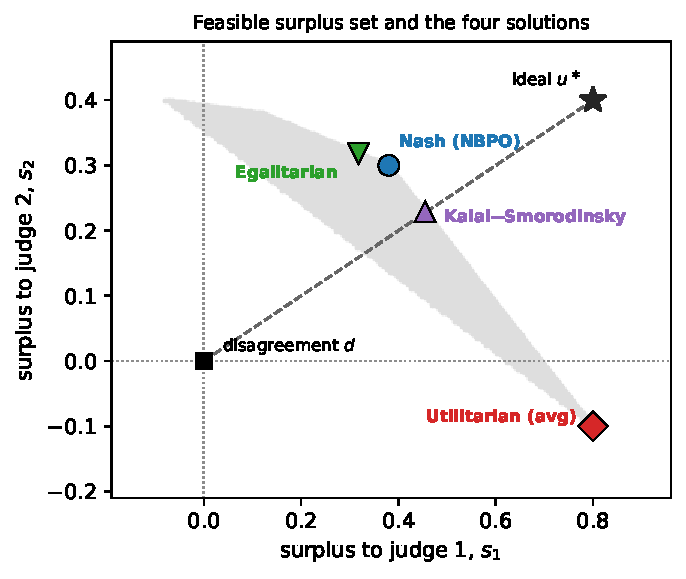
\includegraphics[width=0.5\linewidth]{figures/synthetic_bargain.pdf}
\caption{Feasible surplus set of a two-judge game (grey), with the disagreement point $d$ at the origin and the ideal point $u^\ast$. The utilitarian (averaging) vertex leaves the positive orthant, driving judge~2 below the reference, while the Nash, Kalai--Smorodinsky, and egalitarian solutions stay strictly interior and distinct. Kalai--Smorodinsky lies on the dashed segment from $d$ to $u^\ast$, as its definition requires.}
\label{fig:bargain}
\end{figure}

\section{Judge Instantiation and Preference Labeling}
\label{app:labeling}
The training oracle $P_k$ is a ground-truth reward model that we do not fit: on \textsc{HelpSteer2} the \texttt{ArmoRM} per-attribute heads (helpfulness, correctness, coherence, and verbosity, with conciseness the negated verbosity head), on \textsc{SafeRLHF} the Beaver reward and cost models. For a pair $(y,y')$ objective $k$ prefers the higher-scoring response, so $P_k(y\succ y')\in\{0,\tfrac12,1\}$ is deterministic and exactly skew-symmetric ($P_k(y\succ y')+P_k(y'\succ y)=1$); by \eqref{eq:skew} the disagreement point is $\tfrac12$ in every coordinate with no estimation. Evaluation is kept separate and uses general LLM judges, \texttt{Qwen3-32B} throughout with \texttt{Llama-3.3-70B} and \texttt{Phi-4} for cross-family robustness: each is prompted with an objective-specific rubric, ends its verdict with \texttt{[[A]]}, \texttt{[[B]]}, or \texttt{[[TIE]]} scored $1$, $0$, or $\tfrac12$, and is judged in both orders and averaged, so the evaluation oracle is skew-symmetric as well. Training and evaluation oracles thus come from different model families, and a language-model judge need not be transitive.

\paragraph{Rubrics.}
Each objective is a one-line rubric telling the judge to compare on that attribute alone and ignore the others: helpfulness asks which response better accomplishes the user's stated goal (a refusal with useful alternatives counts as more helpful than a bare refusal), correctness which is more accurate, coherence which is clearer and better organized, conciseness which conveys the same content with less padding (\textsc{HelpSteer2}), and harmlessness which is safer (\textsc{SafeRLHF}).

\paragraph{Helpfulness prompt.}
For concreteness we give the helpfulness prompt verbatim; the other objectives reuse the same template and differ only in the rubric line. The rubric is the system message and the pair is the user message, with $\{$prompt$\}$, $\{$A$\}$, and $\{$B$\}$ filled in per instance and the two responses swapped across the two queries.
\begin{quote}\small\ttfamily
System: You compare two AI responses on HELPFULNESS ONLY: which better helps the user accomplish their stated goal (relevance, substance, actionable detail). Ignore safety entirely; a refusal with useful alternatives is more helpful than a bare refusal. End with exactly [[A]] or [[B]] or [[TIE]].

User: [User prompt] $\{$prompt$\}$ [Response A] $\{$A$\}$ [Response B] $\{$B$\}$ Verdict:
\end{quote}

\paragraph{From verdicts to training targets.}
The anchored surplus of objective $k$ is the swap-averaged win rate of the policy's samples against the reference's, $\hat s_k=u_k(\pi)-\tfrac12$ with $u_k(\pi)=P_k(\pi\succ\mu)$, which is also the anchored utility reported throughout (estimated on held-out prompts). From these surpluses the Nash and Kalai--Smorodinsky weights are formed as in the main text, and every rule (utilitarian, egalitarian, NBPO-NBS, NBPO-KS) together with the baselines (INPO, HT-MNPO) trains on the same judged comparisons through the same regression, differing only in the per-objective weight; no reward model enters at any point.

\end{document}